\documentclass[a4paper,11pt,twocolumn]{article}
\usepackage[a4paper,left=1.5cm,right=1cm,top=2cm,bottom=2cm]{geometry}
\usepackage{setspace}
\usepackage{gensymb}
\usepackage{caption}
\usepackage{graphicx}
\usepackage{tabularx}
\usepackage{lmodern}
\usepackage{watermark} 
\usepackage{lipsum}
\usepackage{xcolor}
\usepackage{listings}
\usepackage{graphicx}
\usepackage{enumitem}
\usepackage{mathtools}
\usepackage{titlesec}
\usepackage[utf8]{inputenc}
\usepackage{fontenc}
\usepackage{harvard}
\usepackage{amsfonts}
\usepackage{tikz}
\graphicspath{{/storage/emulated/0/Download/FWC/Latex/figs}}
\usepackage[colorlinks,linkcolor={black},citecolor={blue!80!black},urlcolor={blue!80!black}]{hyperref}
\title{\textbf{\textsc{VERIFICATION OF BOOLEAN IDENTITIES}}}
\author{\textbf{\textit{\teflipflopxtbf{Rudra Pratap Singh}}}}
\begin{document}

\date{}
\maketitle
\tableofcontents



\section{PROBLEM}
\textbf{(GATE CS-2008)}
\textbf{Q.5} In the Karnaugh map shown below, X denotes a don't care term. What is the minimal form of the function represented by the Karnaugh map?


\tikzset{every picture/.style={line width=0.75pt}} %set default line width to 0.75pt        

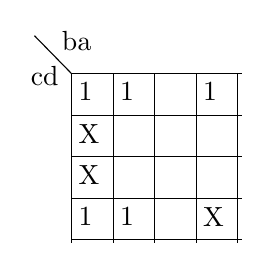
\begin{tikzpicture}[x=0.75pt,y=0.75pt,yscale=-1,xscale=1]
%uncomment if require: \path (0,235); %set diagram left start at 0, and has height of 235

%Shape: Grid [id:dp9981783189121591] 
\draw  [draw opacity=0] (106,41) -- (188,41) -- (188,122.6) -- (106,122.6) -- cycle ; \draw   (106,41) -- (106,122.6)(126,41) -- (126,122.6)(146,41) -- (146,122.6)(166,41) -- (166,122.6)(186,41) -- (186,122.6) ; \draw   (106,41) -- (188,41)(106,61) -- (188,61)(106,81) -- (188,81)(106,101) -- (188,101)(106,121) -- (188,121) ; \draw    ;
%Straight Lines [id:da6508935575311161] 
\draw    (88,22.6) -- (106,41) ;

% Text Node
\draw (108,64) node [anchor=north west][inner sep=0.75pt]   [align=left] {X};
% Text Node
\draw (108,84) node [anchor=north west][inner sep=0.75pt]   [align=left] {X};
% Text Node
\draw (168,104) node [anchor=north west][inner sep=0.75pt]   [align=left] {X};
% Text Node
\draw (100,19) node [anchor=north west][inner sep=0.75pt]   [align=left] {ba};
% Text Node
\draw (85,36) node [anchor=north west][inner sep=0.75pt]   [align=left] {cd};
% Text Node
\draw (108,104) node [anchor=north west][inner sep=0.75pt]   [align=left] {1};
% Text Node
\draw (168,44) node [anchor=north west][inner sep=0.75pt]   [align=left] {1};
% Text Node
\draw (108,44) node [anchor=north west][inner sep=0.75pt]   [align=left] {1};
% Text Node
\draw (128,44) node [anchor=north west][inner sep=0.75pt]   [align=left] {1};
% Text Node
\draw (128,104) node [anchor=north west][inner sep=0.75pt]   [align=left] {1};


\end{tikzpicture}
\begin{enumerate}[label=(\Alph*)]
	\item $ b'd'+a'd' $
	\item $ a'b'+b'd'+a'bd' $
	\item $ b'd'+a'bd' $
	\item $ a'b'+b'd'+a'd' $
 
        


\tikzset{every picture/.style={line width=0.75pt}} %set default line width to 0.75pt        

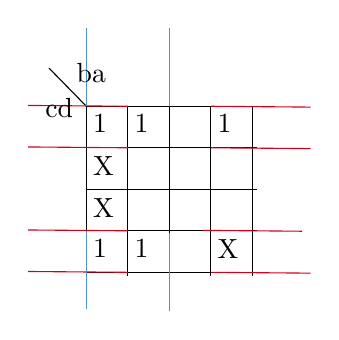
\begin{tikzpicture}[x=0.75pt,y=0.75pt,yscale=-1,xscale=1]
%uncomment if require: \path (0,235); %set diagram left start at 0, and has height of 235

%Shape: Grid [id:dp9981783189121591] 
\draw  [draw opacity=0] (106,41) -- (188,41) -- (188,122.6) -- (106,122.6) -- cycle ; \draw   (106,41) -- (106,122.6)(126,41) -- (126,122.6)(146,41) -- (146,122.6)(166,41) -- (166,122.6)(186,41) -- (186,122.6) ; \draw   (106,41) -- (188,41)(106,61) -- (188,61)(106,81) -- (188,81)(106,101) -- (188,101)(106,121) -- (188,121) ; \draw    ;
%Straight Lines [id:da6508935575311161] 
\draw    (88,22.6) -- (106,41) ;
%Straight Lines [id:da9264334067048627] 
\draw [color={rgb, 255:red, 208; green, 2; blue, 27 }  ,draw opacity=1 ]   (78,60.6) -- (126,61) ;
%Straight Lines [id:da6733319746718234] 
\draw [color={rgb, 255:red, 208; green, 2; blue, 27 }  ,draw opacity=1 ]   (78,40.6) -- (126,41) ;
%Straight Lines [id:da46034895503597606] 
\draw [color={rgb, 255:red, 208; green, 2; blue, 27 }  ,draw opacity=1 ]   (78,100.6) -- (126,101) ;
%Straight Lines [id:da4662868353575773] 
\draw [color={rgb, 255:red, 208; green, 2; blue, 27 }  ,draw opacity=1 ]   (78,120.6) -- (126,121) ;
%Straight Lines [id:da10918253437593739] 
\draw [color={rgb, 255:red, 208; green, 2; blue, 27 }  ,draw opacity=1 ]   (166,121) -- (214,121.4) ;
%Straight Lines [id:da08354527188381211] 
\draw [color={rgb, 255:red, 74; green, 144; blue, 226 }  ,draw opacity=1 ]   (106,138.6) -- (106,101) ;
%Straight Lines [id:da8351403004315967] 
\draw [color={rgb, 255:red, 208; green, 2; blue, 27 }  ,draw opacity=1 ]   (166,61) -- (214,61.4) ;
%Straight Lines [id:da8509450418900439] 
\draw [color={rgb, 255:red, 208; green, 2; blue, 27 }  ,draw opacity=1 ]   (166,41) -- (214,41.4) ;
%Straight Lines [id:da8468684734891763] 
\draw [color={rgb, 255:red, 208; green, 2; blue, 27 }  ,draw opacity=1 ]   (162,100.8) -- (210,101.2) ;
%Straight Lines [id:da2686725260803322] 
\draw [color={rgb, 255:red, 74; green, 144; blue, 226 }  ,draw opacity=1 ]   (146,41) -- (146,3.4) ;
%Straight Lines [id:da627292688010811] 
\draw [color={rgb, 255:red, 74; green, 144; blue, 226 }  ,draw opacity=1 ]   (106,41) -- (106,3.4) ;
%Straight Lines [id:da14905829603237186] 
\draw [color={rgb, 255:red, 74; green, 144; blue, 226 }  ,draw opacity=1 ]   (146,139.8) -- (146,102.2) ;

% Text Node
\draw (108,64) node [anchor=north west][inner sep=0.75pt]   [align=left] {X};
% Text Node
\draw (108,84) node [anchor=north west][inner sep=0.75pt]   [align=left] {X};
% Text Node
\draw (168,104) node [anchor=north west][inner sep=0.75pt]   [align=left] {X};
% Text Node
\draw (100,19) node [anchor=north west][inner sep=0.75pt]   [align=left] {ba};
% Text Node
\draw (85,36) node [anchor=north west][inner sep=0.75pt]   [align=left] {cd};
% Text Node
\draw (108,104) node [anchor=north west][inner sep=0.75pt]   [align=left] {1};
% Text Node
\draw (168,44) node [anchor=north west][inner sep=0.75pt]   [align=left] {1};
% Text Node
\draw (108,44) node [anchor=north west][inner sep=0.75pt]   [align=left] {1};
% Text Node
\draw (128,44) node [anchor=north west][inner sep=0.75pt]   [align=left] {1};
% Text Node
\draw (128,104) node [anchor=north west][inner sep=0.75pt]   [align=left] {1};


\end{tikzpicture}
\bigskip
                        
 One group consists of (0000, 0010, 1000, 1010) which gives b’d’
 Other group is (0000, 0001, 1000, 1001) which gives a’d’ So, solution is b’d’ + a’d’.
 Hence  ,  correct option is a).



\end{enumerate}
\bigskip

\section{COMPONENTS}
	\begin{tabularx}{0.45\textwidth} {  
  | >{\centering\arraybackslash}X  
  | >{\centering\arraybackslash}X  
  | >{\centering\arraybackslash}X | } 
\hline 
\textbf{Component} &  \textbf{Value} & \textbf{Quantity}\\ 
\hline 
Arduino & UNO & 1 \\   
\hline 
Bread board & - & 1 \\ 
\hline
Jumper wires & M-M & 10 \\ 
\hline 
LED & - & 1\\ 

\hline 
\end{tabularx}
 
\bigskip 

\section{TRUTH TABLE}
The Truth Table for the identity is as follows:
\begin{enumerate}[label=\textbf{(\Alph*})]
	\item \textbf{ $ Y=b'd'+a'd' $} \\
\bigskip
\begin{table}[ht!]
	\centering
\begin{tabular}{ |c |c |c |c |c |c |} 
\hline 
\newline 
	\textbf{a} & \textbf{b} & \textbf{d} & \textbf{Y} \\ 
\hline  
	0 & 0 & 0 &1 \\   
	0 & 0 & 1 &0 \\  
	0 & 1 & 0 &1 \\  
	0 & 1 & 1 &0 \\  
	1 & 0 & 0 &1 \\  
	1 & 0 & 1 &0 \\  
	1 & 1 & 0 &0 \\  
	1 & 1 & 1 &0 \\  
\hline 
\end{tabular}
	\caption{}
\end{table}
\bigskip
\bigskip


\end{enumerate}
\section{ARDUINO CONNECTIONS}

1) The connections taken from Arduino as Input and Output is as follows:
\begin{table}[ht!] 
    \centering 
    \begin{tabular}{|c|c|c|c|c|c|c|c|} 
    \hline 
       Input & $a$&$b$&$d$&$Y$\\ 
       \hline 
    Arduino & 3&4&5&6\\ 
    \hline 
    \end{tabular} 
    \caption{} 
\end{table} 
\\
2) The  input \textbf{a,b,c} here are connected to Arduino D3,D4,D5 pins.\\
3) The  output \textbf{Y} here are connected to Arduino D6 pins.\\
4) The values for these inputs are conncted either to GND or 5V according to the truth table.\\
\section{CODE}
\paragraph{}
	The arduino code can be downloaded from the below link.
\begin{center} 
\fbox{\parbox{8.5cm}{\url{https://github.com/Rudrapratap1404/Rudrapratap1404/blob/main/Arduino/src/code.ino}}} 
\end{center}


\end{document}
